\begin{figure}[htbp]
\centering
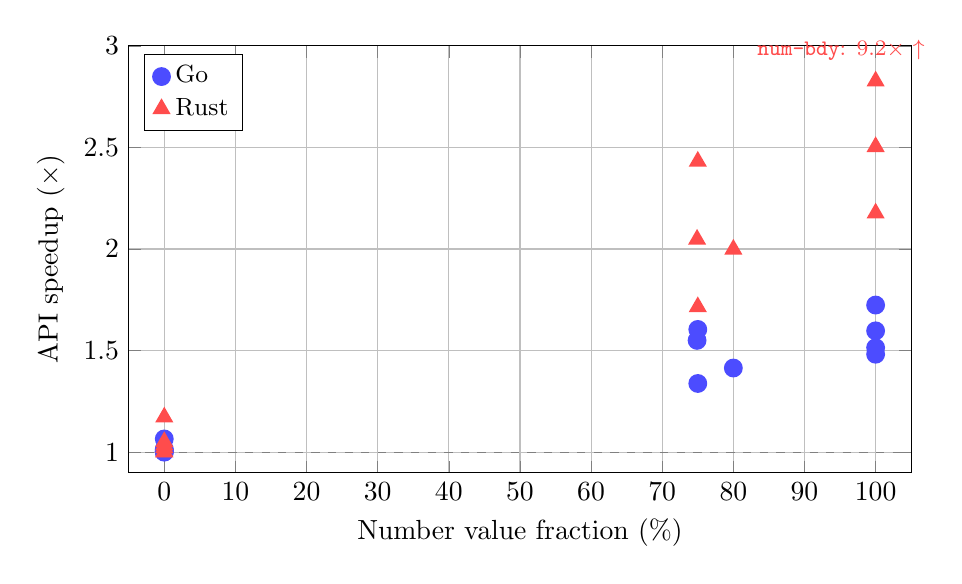
\begin{tikzpicture}
\begin{axis}[
    width=0.95\columnwidth,
    height=7cm,
    xlabel={Number value fraction (\%)},
    ylabel={API speedup ($\times$)},
    xmin=-5, xmax=105,
    ymin=0.9, ymax=3.0,
    grid=major,
    legend style={at={(0.02,0.98)}, anchor=north west, font=\small},
    legend cell align={left},
    mark size=3pt,
    clip=false,
]
% Go API speedups (workload order: deep-64, long-string, unicode,
% surrogate-pair, rfc-key-sorting, control-escapes, small, nested-mixed,
% numeric-boundary, canonical-minimal, array-256, array-2048,
% escaped-key-order, verify-whitespace)
\addplot[only marks, mark=*, blue!70, thick] coordinates {
    (0.0, 1.000)
    (0.0, 1.003)
    (0.0, 1.002)
    (0.0, 1.015)
    (0.0, 1.010)
    (0.0, 1.065)
    (75.0, 1.338)
    (80.0, 1.414)
    (100.0, 1.482)
    (100.0, 1.514)
    (74.9, 1.550)
    (75.0, 1.604)
    (100.0, 1.597)
    (100.0, 1.724)
};
% Rust API speedups (excluding numeric-boundary 9.19x outlier)
\addplot[only marks, mark=triangle*, red!70, thick] coordinates {
    (0.0, 1.021)
    (0.0, 1.001)
    (0.0, 1.172)
    (0.0, 1.051)
    (0.0, 1.035)
    (0.0, 1.000)
    (75.0, 1.715)
    (80.0, 1.998)
    (100.0, 2.176)
    (74.9, 2.047)
    (75.0, 2.431)
    (100.0, 2.503)
    (100.0, 2.826)
};
\legend{Go, Rust}
% Annotation for numeric-boundary (off-chart at 100%, 9.19x)
\node[anchor=south west, font=\footnotesize, red!70] at (axis cs:82,2.88)
    {\texttt{num-bdy}: 9.2$\times$ $\uparrow$};
% Reference line at 1.0x (no effect)
\draw[dashed, gray, thin] (axis cs:-5,1.0) -- (axis cs:105,1.0);
\end{axis}
\end{tikzpicture}
\caption{Relationship between workload number value fraction and API
speedup of \schubfach over \burgerdybvig (canonicalize mode).  Workloads
with zero number content cluster near 1.0$\times$ (no algorithmic
difference); number-dense workloads ($>$70\%) show 1.3--1.7$\times$ in
Go and 1.7--2.8$\times$ in Rust.  The Rust
\texttt{numeric-boundary} outlier (9.2$\times$) is annotated but
excluded from the $y$-axis range.}
\label{fig:density-speedup}
\end{figure}
